\setchapterpreamble[u]{%
\dictum[Sokrates]{Hast du etwas Schwieriges zu erledigen, beauftrage damit einen Faulen. Er wird einen leichten Weg finden, es auszuführen. \dots}}
\chapter{Aufgabenbeschreibung} \index{Aufgabenbeschreibung}\label{kap:aufgabenbeschreibung}

\section{Problemstellung}\label{sec:problemstellung}
%\todotext{Problemstellung ausformulieren: 
%Was ist das Problem? 
%• Warum ist es wichtig? 
%• Warum ist es nicht trivial? 
%• Was möchte ich zur Lösung beitragen beitragen? 
%}

%Was ist das Problem, aktuelle Situation?
%Automatisierter Datenaustausch von Produktdaten in der Industrie, konkretes Problem Abfrage der Produktdaten und Antwort. 

Der automatisierte Austausch von Produktdaten spielt in der Geschäftswelt eine enorm große Rolle. Es fallen in der Industrie, der Wissenschaft, der Gesellschaft große Datenmengen an wie z.B. die Daten von Produkten, Bestellungen, Rechnungen, Lieferungen oder in der Verwaltung von Personen. Der elektronische Datenaustausch erfolgt in der Regel nach einem festem Schema. Hierbei ist das Austauschformat sowie die Schnittstelle über die diese Daten ausgetauscht werden dem Anfragenden als auch dem Anbieter festgelegt und bekannt. Man \enquote{einigt} sich auf definierte Schema. Dazu nutzt man definierte Standards. Geben die Parteien an, die Anforderungen an einen öffentlichen Standard zu erfüllen, sind diese Parteien in der Lage über diesen Standard Daten auszutauschen. Mit Hilfe dieser Standards werden Geschäftsprozess definiert, um beispielsweise den Austausch der Daten zu realisieren. Diese wohldefinierten Prozesse in der Geschäftswelt sind in der Regel sehr unflexibel. Dadurch, dass das Modell der Daten sowie die Schnittstelle \enquote{fest verdrahtet} ist, bedeuten beispielsweise Änderungen in den Anforderungen nach Inhalten der Daten meistens eine Änderung des Modells, gleichsam der auszutauschenden Daten mit Ihren Eigenschaften, als auch eine Anpassung der Schnittstelle. 

%Beispiele für relationen algebra in latex
%Query \verb$SELECT x.a FROM x,y,z WHERE x.a=y.a OR x.a=z.a$
%$\Pi_{x.a} ((x \Join y)\cup(x \Join z))$.
%$temp1 \leftarrow (customer \times account) $ \\
%$temp2 \leftarrow  \sigma_{(customer.sin = account.sin}(temp1)$ \\
%$basic-cust-accts \leftarrow \Pi_{(name, customer.sin, account-number)} (temp2) $ \\
%$basic-cust-accts \leftarrow \Pi_{(name, customer.sin, account-number)} (\sigma_{customer.sin = account.sin}(customer \times account))$

Um das Problem zu lösen bieten sich flexible Mechanismen einer Abfrage- und Antwortschnittstelle an. Herkömmlicherweise wird dann diese Schnittstelle anbieterseitig implementiert. Dann werden Methoden angeboten, welche diese Abfragen ermöglichen und passend zu diesen Abfragen entsprechende Antworten mit den gewünschten Daten erzeugt. 
Diese herkömmlichen Datenaustauschmechanismen einigen sich somit auf eine Schnittstelle, auf ein Schema und sind somit gekoppelt an das Modell. Die flexiblen Abfragemechanismen sind anbieterseitig nahe der Datenquelle implementiert, zumeist bereit implizit vorhanden, beispielsweise durch ein Datenbanksystem mit einer SQL\footnote{Standard Query Language - Abfragesprache für relationale Datenbanken}-Abfrageschnittstelle. 
Eine weitere zusätzliche Metaebene hingegen ermöglicht einen flexiblen und standardisierten Datenaustausch, wobei die tatsächlichen Werte der Daten vom Modell abgekoppelt sind. Der Vorteil dieser Lösung ist, dass diese Abfrage- und Antwortschnittstelle auf Schemaebene lose gekoppelt von der tatsächlichen Implementierung ist. 

Der ISO Standard 29002-31 beschreibt eine solche Abfrage- und Antwortschnittstelle für Produktdaten. Diese ermöglicht den flexiblen automatisierten Austausch von Produktdaten. Diese Daten (Master Data) werden abgekoppelt von der Semantik abgefragt. Die Semantik wird mittels Konzepten beschrieben. Auf diese Konzepte wird mittels eindeutigem Identifier referenziert. 

\section{Zielsetzung}

Es soll eine Abfrageschnittstelle (Query-Schnittstelle) für die bereits vorhandene PLIB\footnote{Parts Library - Implementierung nach ISO-13584}  des Fachbereiches erstellt werden. 

Diese Abfrageschnittstelle soll die Standards der ISO 29002-31, sowie für deren Nutzung gegebenenfalls weitere nötige Standards unterstützen. Diese Schnittstelle soll einen automatisierten Datenaustausch ermöglichen und technisch auf den Abfrageprozeduren der Datenbankebene basieren. Die Implementierung dieser Prozeduren und des Datenbankschemas ist Teil der Arbeit zweier Kommilitonen (Herr Mende und Herr Loth).
 
Das Hauptziel ist die Machbarkeit und die Integration der ISO-Schnittstelle aufbauend auf die vorhandene PLIB Datenbankimplementierung des Fachbereiches aufzuzeigen. 
Ferner ist mit aktuellen Techniken eine Integration, gleichsam Nutzbarkeit der Abfrage der Datenbank zu ermöglichen. Wichtig ist es, die gegebenen ISO Normen zu unterstützen, um Wiederverwendbarkeit zu gewährleisten. Falls Teile der Implementierung von den ISO Normen abweichen oder die Standards erweitert oder geändert werden, wird darauf mit ausführlicher Erläuterung der Gründe hingewiesen. 


Um das Ziel zu erreichen, soll im Rahmen der Arbeit untersucht werden welche mögliche sinnvollen Anwendungsfälle sich in der Praxis basierend auf den zu unterstützenden ISO Standards ergeben. Dafür ist eine Analyse der Standards nötig, um zu prüfen, ob und in welcher Form die flexiblen Abfragemöglichkeiten unterstützt werden. Wie in \autoref{sec:problemstellung} erwähnt, gibt es auf Datenbankebene oft eine implizite Abfrageschnittstelle, welche in SQL realisiert ist. Es bietet sich daher an, die Möglichkeiten von SQL-Abfragen als Basis für die Untersuchung zu nehmen, und zu prüfen welche Abfragen mit Hilfe des Standards realisiert werden können. 
Betrachtet werden soll die Projektion und die Selektion.

\begin{description}
\item[Projektion] Die Attributbeschränkung gleichsam einer \enquote{Spaltenauwahl} in relationalen Datenbanken. In SQL das \enquote{select} Keyword.   

In Relationenalgebra:
$ergebnisprojektion \leftarrow  \Pi_{(attribut_1, attribut_2... attribut_n)}(plib)$ \\

\item[Selektion] Schränkt eine Suche mittels Prädikaten ein auf passende Tupel, gleichsam einer \enquote{Zeilenauswahl}. In SQL das \enquote{where} Schlüsselwort samt Mengenoperatoren, wie z.B. \enquote{UND, ODER, NICHT}.

In Relationenalgebra:
$ergebnis-selektion \leftarrow  \sigma_{(praedikat_1, praedikat_2... praedikat_n})(plib)$ \\

\end{description}

Für die Schnittstelle ist eine prototypische Implementierung zu erstellen. Weiterer Bestandteil der Arbeit ist unter Beachtung der technischen Vorgaben, eine Beschreibung des Auswahlprozesses der Techniken, Plattform, Architektur und Programmiersprachen. Die Vor- und Nachteile der einzelnen Optionen des Auswahlprozesses und weitere Nutzungs-, respektive Erweiterungs- und Integrationsmöglichkeiten der entwickelten Schnittstelle sind zu erläutern. 
Die Entwicklung der Software soll nach einem aktuell üblichen Softwareentwicklungsprozess erfolgen. 

\section{Details und Abgrenzung}

\subsection{Gesamtkontext der PLIB Abschlussarbeiten}

Um einen Überblick zu schaffen in welchem Kontext sich diese Arbeit befindet und den Gesamtzusammenhang zu verstehen, soll hier eine kurze Übersicht über die PLIB Abschlussarbeiten des Fachbereiches geschaffen werden. 

%\bild{gesamtkontext_plib}{16cm}{gesamtkontext_plib}{gesamtkontext_plib}

\begin{figure}[htbp]
	\centering
		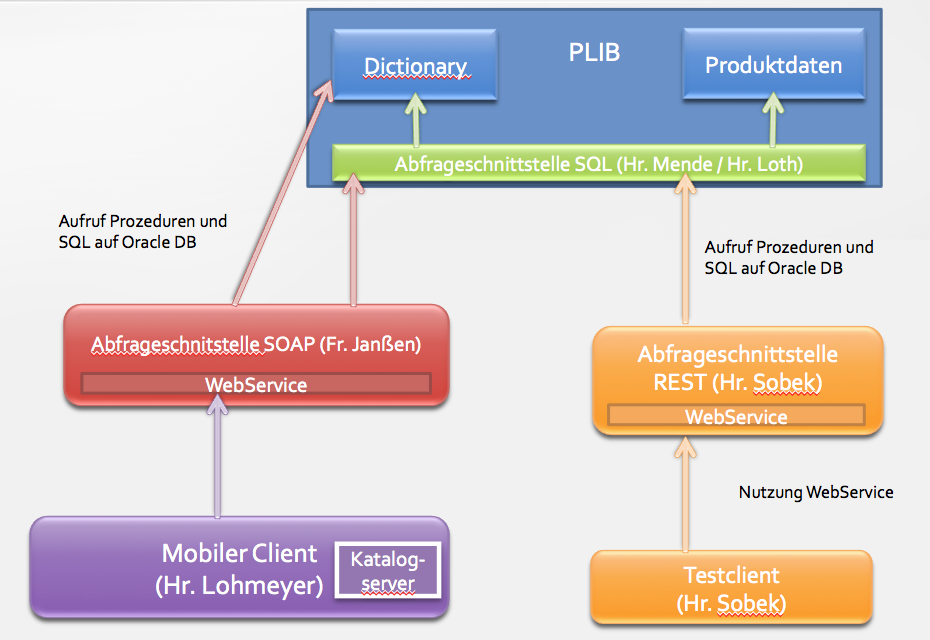
\includegraphics[width=0.98\textwidth]{images/gesamtkontext_plib.png}
	\caption{Gesamtkontext PLIB Abschlussarbeiten}
	\label{fig:gesamtkontext_plib}
\end{figure}

Die \autoref{tab.gesamtkontext} erläutert die \autoref{fig:gesamtkontext_plib} und listet dazu die auf die jeweiligen Arbeiten basierenden ISO-Standards auf: 

% \cellcolor{<Farbe>}, \rowcolor{<Farbe>}, {\columncolor{<Farbe>}}, ändern die Hintergrundfarbe. 
\begin{table}[!hbt]\vspace{1ex}\centering
\scriptsize
\begin{tabular}{p{3.15cm}p{2.8cm}p{5.5cm}p{3cm}}
\toprule \rowcolor{mylightergray}
\textbf{Bezeichnung} & \textbf{Arbeit von} & \textbf{Erläuterung} &  \textbf{ISO Standards}\\
\midrule
Abfrageschnittstelle als Web Service mit SOAP &  Frau Janßen & Implementierung eines Webservices zur Auflösung von Konzept-Identifikatore in Konzept-Dictionaries/Ontologien & ISO 29002-20 \\
\hline
PLIB, Dictionary und Produktdatenbank &  Herr Mende und Herr Loth & Meta- und Produktdatenbank  sowie eine Abfrageschnittstelle basierend auf Oracle. Entwicklung von Abfrageschnittstellen mit Oracle Prozeduren & ISO 13584-42 \citep[Vergl.][]{iso13584-42}  \\
\hline
Mobiler Abfrageclient & Herr Lohmeyer & Entwicklung eines mobilen Abfrageclients basieren auf Android. Der Client nutzt die Web Servcies von Frau Janßen und beinhaltet einen eigenen Katalogserver. & ISO 29002-10, ISO 13584-42 \\
\hline
Abfrageschnittstelle als Web Service mit REST für Charakteristische Produktdaten & Herr Sobek & Entwicklung einer Schnittstelle zur Abfrage von Charakteristischen Produktdaten. Die Schnittstelle wird als RESTful Web Service implementiert. & ISO 29002-31, ISO 29002-10 \\
\bottomrule
\end{tabular}
\caption{\label{tab.gesamtkontext}Erläuterung der Gesamtkontextabbildung}
\vspace{2ex}\end{table}

\subsection{Abgrenzung}

Die Arbeit umfasst die Implementierung der Use Cases nach \autoref{kap:Use_Cases}. Dies beinhaltet im wesentlichen den Teil 31 der ISO 29002 - einen Abfragestandard für Charakteristische Produktdaten. 
Weiterhin wird für die Datenübertragung eine Implementierung des Teils 10 der ISO 29002 benötigt, siehe \autoref{fig:lieferketten}. 
Die Arbeit befasst sich nicht mit der Implementierung eines Identification Guides nach ISO 22745-30. Dieser wird in der Praxis von einem Klienten für eine sinnvolle Vorauswahl der für sich oder seine Organisation benötigten Attribute der Teile verwendet. Jeder Klient definiert für seinen Kontext sinnvolle Attribute und Teiledaten und definiert diese mit Hilfe des Schemas der ISO 22745-30. Dies kann mittels eines Webformular auf Klientseite erfolgen oder als allgemeines Formular mit z.B. Excel\footnote{Excel ist ein bekanntes Tabellenkalkulationsprogramm der Firma Microsoft}, welches die für den/die Klienten relevanten Attribute der Produkte enthält die abgefragt werden sollen. Für mehr Informationen zum Identification Guide siehe \autoref{kap:identification_guide}.

%Beispiel: bild mit footnote
\begin{figure}[htbp]
	\centering
		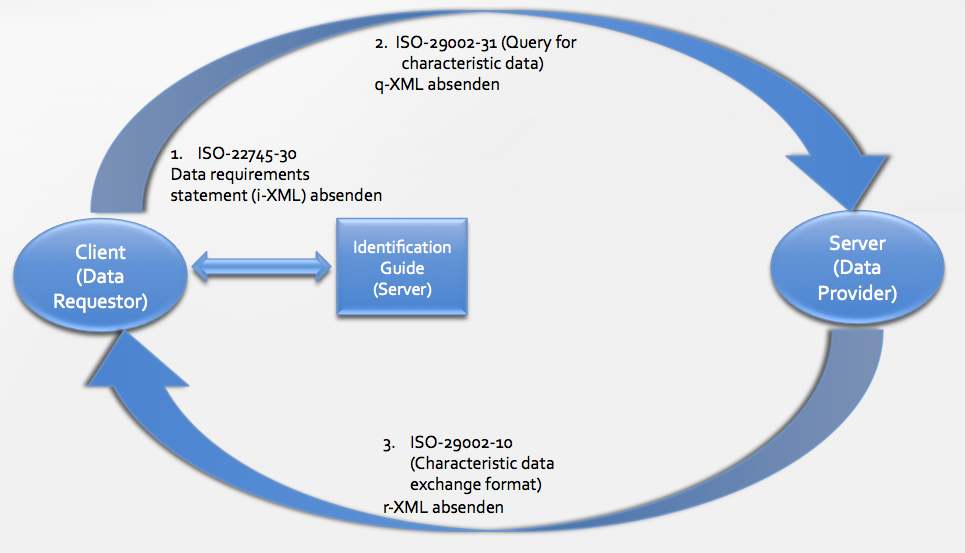
\includegraphics[width=0.99\textwidth]{images/lieferketten_plib.png}
		\caption[Lieferketten]{Lieferketten\footnotemark}
	\label{fig:lieferketten}
\end{figure}
\footnotetext{Abbildung entnommen und abgewandelt aus Benson, Converting Standard Terminology into usable Metadata, 2008 - später in ähnlicher Form auch in Uiterwyk, Die Bedeutung der Merkmalleisten bei eCl@ss, 2012 zu finden.}

\subsection{Vorgaben}

Für die Implementierung sind folgende nichtfunktionale Anforderungen vom Fachbereich vorgegeben:
\begin{description}
\item[Datenbanksystem Oracle] Dieses beinhaltet die PLIB Datenbank samt Abfrageprozeduren und stellt als Teiledatenbank die Basis dar. Dies wird vom Fachbereich bzw. von den Studenten Herr Mende/Herr Loth gestellt. Für die Entwicklung dieses Prototypen wird eine Version von Herrn Mende vom \todotext{Versionsdatum von der PLIB von Karsten Mende einfügen} benutzt.  
\item[Web Services] Auf Grund der hohen Verbreitung und Integrationsmöglichkeiten soll die Schnittstelle als Web Service entwickelt werden. Die ISO 29002-31 schlägt als Beispiel eine E-Mail Schnittstelle vor, dies ist aber keine Vorgabe. Siehe Abbildung \autoref{fig:datenfluesse}, welche besagt:
\begin{quotation}
Transport: not specified in ISO/TS 29002 (could use email) Payload XML.Query XML schema in ISO/TS 29002-31
\end{quotation}
\item[PLIB Datenbankprozeduren] Die vorhandenen Prozeduren zum Zugriff auf die PLIB Datenbank sollen so weit wie möglich verwendet werden. 
\end{description}

\subsection{Datenflüsse}
Das System soll einen \gls{Webservice} zur Verfügung stellen. Dieser \gls{Webservice} soll eine XML Datei gemäß ISO 29002-31 entgegennehmen. Die entsprechende Verarbeitung des XMLs, sowie die logische Transformation der Anfrage zur Abfrageschnittstelle der Datenbank wird vom System vorgenommen. Die Antwort der Datenbank soll wieder zurücktransformiert werden und als Katalog-XML Datei gemäß ISO 29002-10 zurückgeliefert werden.
 
Der gerahmte Bereich im unteren Teil der \autoref{fig:datenfluesse} zeigt in der Datenflussabbildung was implementiert werden soll. Das Zielsystem, gleichsam das System welches die Anfrage erhält wird hier als \enquote{Catalogue Server bezeichnet}. 
Die Kommunikation des Klienten mit dem Location Server, Terminology Server und dem Ontology Server ist Teil der Abschlussarbeit von Fr. Janßen \citep[Vergl.][]{janssen}. 
Die Abfrageprozeduren des Katalogservers auf Datenbankebene ist Aufgabe von Herrn Mende. Zur Zeit der Abgabe dieser Arbeit, war die Arbeit von Herrn Mende noch in Bearbeitung\footnote{Die die Basis dieser Abschlussarbeit ist ein stabiler Implementierungsstand, welcher von Herrn Mende geliefert wurde}. 

\begin{figure}[htbp]
	\centering
		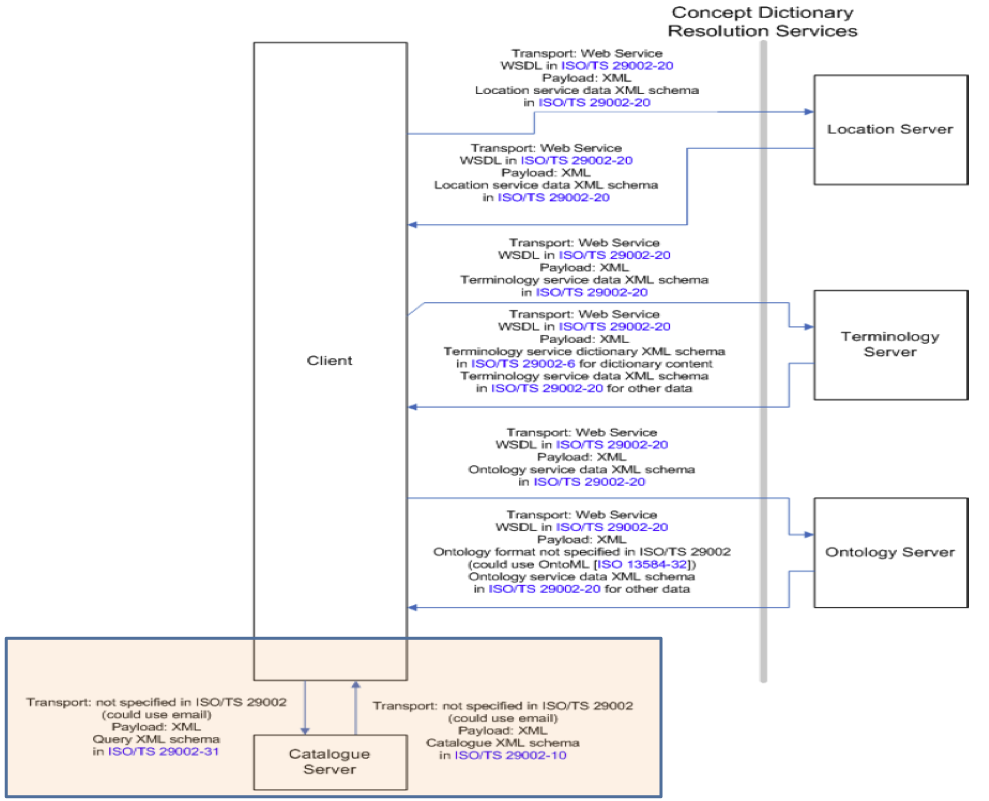
\includegraphics[width=0.99\textwidth]{images/datenfluesse_plib.png}
	\caption[Datenflüsse]{Datenflüsse\footnotemark}
	\label{fig:datenfluesse}
\end{figure}
\footnotetext{Quelle: entnommen ISO 29002-31 Figure 3 - Major Dataflows. Zu besseren Visualisierung wurde der untere Bereich farblich hervorgehoben.}
